\documentclass{article} % Oder eine andere Dokumentklasse wie report, book, etc.
\usepackage[utf8]{inputenc} % Bestimmt die Eingabe-Kodierung
\usepackage[T1]{fontenc} % Bestimmt die Ausgabe-Kodierung
\usepackage{graphicx}


\begin{document}
	
	\title{Deep Reinforcement Learning Exercise 02}
	\maketitle
	
	\section{Exercise 2.1}
	We implemented the grid as a 5x5 matrix using np.array. We also tried to follow the gym library class, by using the functions __init__, step, reset and render (which we really didnt need in this exercise). 
	\subsection{2.1a}
	We implemented the function state_value_iteration_bellman by looping over all the grid cells and computing the state value according to the bellman equation, while handling the "jumping" of the agent for the special states. 
	The plot shows all the state values over time, as well as the state values at the final iteration, using a colormap. As expected, the cells close to the ones, where a positive reward is given, have a quite high state value, and the ones on the bottom of the grid have low state values, with the worst even being negative. 
	As we can see, the state values converge after 10-20 iterations. Since we are using a random policy, the state values cannot change after a couple of iterations, since we are not learning anything. 
	\subsection{2.1b}
	We implemented the function action_value_iteration_bellman by looping over all grid cells and each action for that grid cell and computing the action value according to the bellman equation. 
	The plots show the action values for all 4 possible direction and each grid cell, as well as all action values over time. Similarily to the first plots, we see high action values for moves onto the cells, which give out the reward, and low action values for the ones moving away from them, with the worst ones also having a negative value. 
	Again, the action values converge after 10-20 iterations, since the random policy doesn't adjust any actions. 

	The differences between both computations is, that you also have to iterate over all actions, so the number of action values is num_actions times that of the state values. Other than that, there are no big differences in writing, as far as we can tell. 
	
	
	\section{Exercise 2.2}
	\subsection{2.2.a}
	Nothing much to be said here to be honest. Please note that we kind of failed to understand the urgency of the function "render(mode)". Since it did not hinder the implementation (2.2 b), we did not further investigate but will be delightet to hear about its functionality in the exercise review :D 
	
	EDIT: Nevermind, just read the functionality on the documentation. Would still be nice to see a working example of the "rendering" and its different modes regarding our task.
	
	Furthermore, we discussed what an episode "ending" in this circumstance would entain? It could be the first teleport, n amount of steps or a certain reward threshold (and many more arbitrary events).
	
	\subsection{2.2.b}
	Again, nothing much to be explained. Implementation worked as expected. We can see the "teleport" upon reaching grid space [0,1] in step 12. 
	
	\begin{figure}[h!]
		\centering
		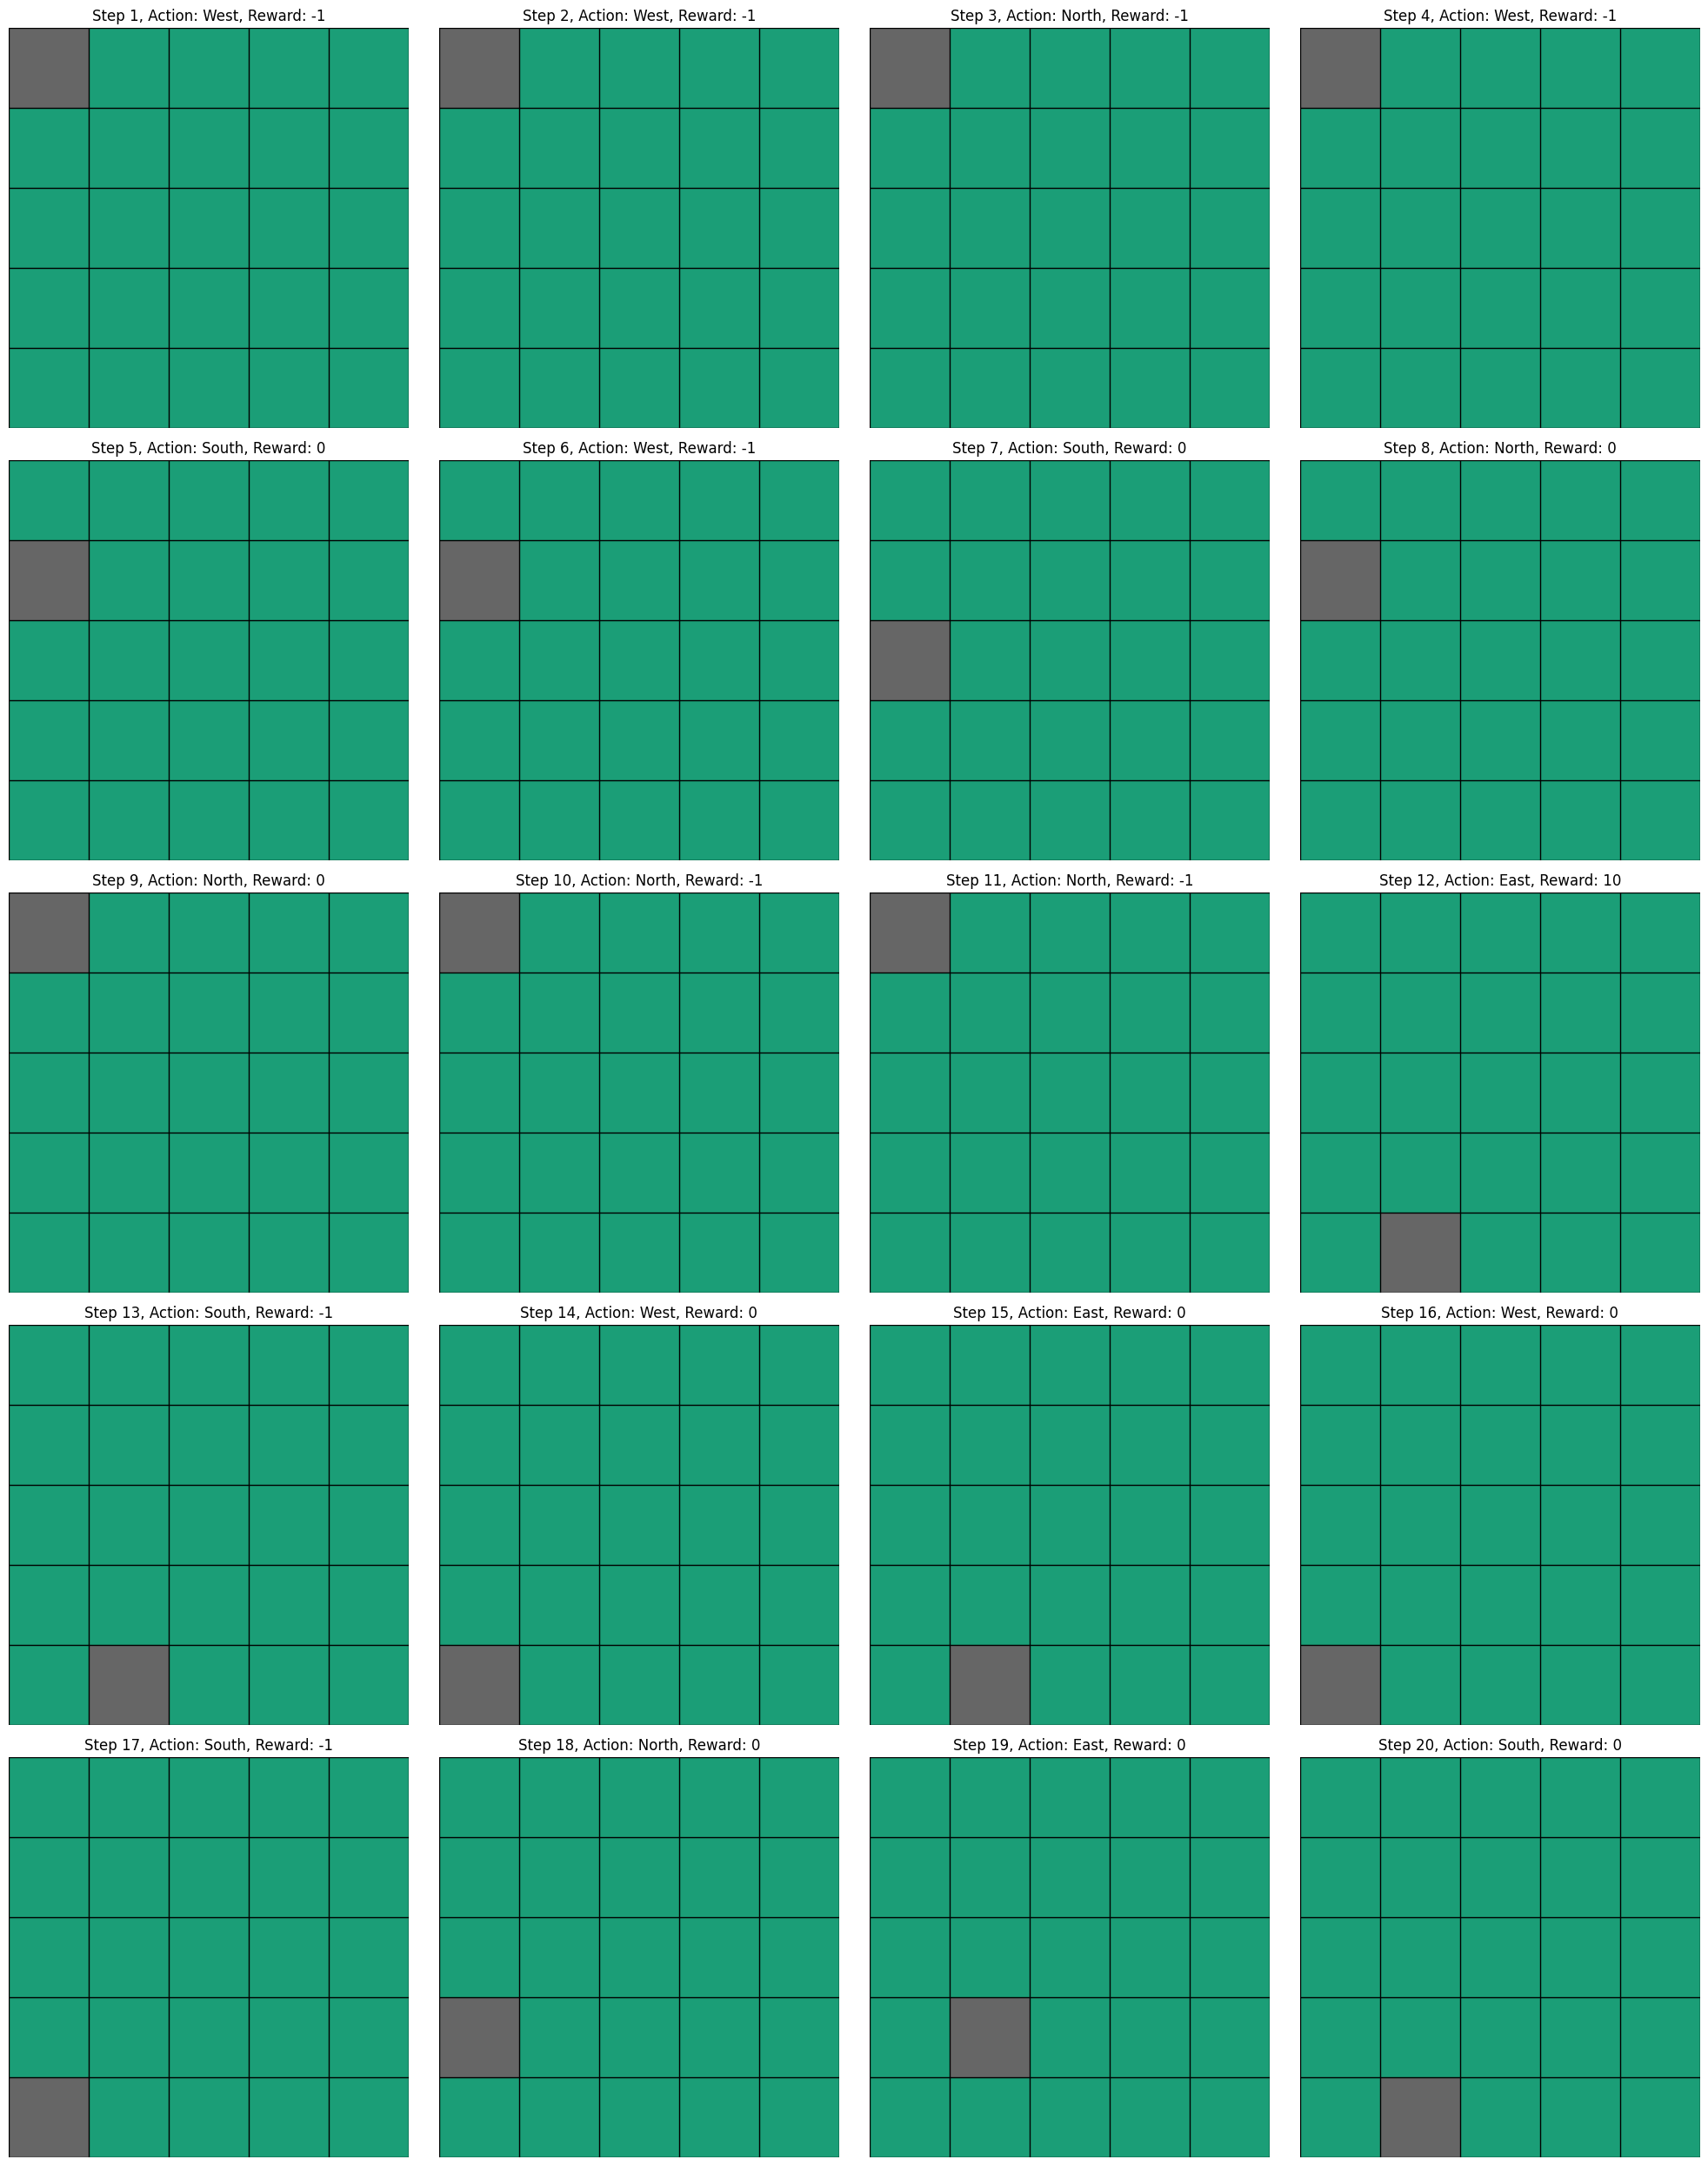
\includegraphics[width=0.9\textwidth]{images/20_steps.png}
		\caption{20 successive steps of the environment}
		\label{fig:1.1.a.1}
	\end{figure}
	
	\end{document}